\documentclass{article}
\usepackage[
        a4paper,% other options: a3paper, a5paper, etc
        left=3cm,
        right=3cm,
        top=3cm,
        bottom=4cm,
        % use vmargin=2cm to make vertical margins equal to 2cm.
        % us  hmargin=3cm to make horizontal margins equal to 3cm.
        % use margin=3cm to make all margins  equal to 3cm.
]{geometry}
%\usepackage[utf8x]{inputenc}
\usepackage{graphicx}
\usepackage{caption}
\usepackage{enumerate}
\usepackage{subcaption}
\usepackage[procnames]{listings}
\usepackage{color}
\usepackage{amssymb}
\usepackage{amsmath}
\usepackage{comment}
\usepackage{hyperref}
\usepackage{blindtext}
\usepackage[titletoc,title]{appendix}
\usepackage{float}
\usepackage{fullpage}
\definecolor{codegreen}{rgb}{0,0.6,0}
\definecolor{codegray}{rgb}{0.5,0.5,0.5}
\definecolor{codepurple}{rgb}{0.58,0,0.82}
\definecolor{backcolour}{rgb}{0.95,0.95,0.92}

\lstdefinestyle{mystyle}{
    backgroundcolor=\color{backcolour},
    commentstyle=\color{codegreen},
    keywordstyle=\color{magenta},
    numberstyle=\tiny\color{codegray},
    stringstyle=\color{codepurple},
    basicstyle=\ttfamily,
    breakatwhitespace=false,
    breaklines=true,
    captionpos=t,
    keepspaces=true,
    numbers=left,
    numbersep=5pt,
    showspaces=false,
    showstringspaces=false,
    showtabs=false,
    tabsize=2
}

\lstset{style=mystyle, language=Matlab}

\renewcommand{\thesection}{\large{Exercise \arabic{section}}}

\title{Computer Vision - Lab 3}
\author{Luuk Boulogne (s2366681) \and Steven Bosch (s1861948)}
\date{\today}

\begin{document}
\maketitle

\section{}
We use the imshow function in Matlab to select the pixels of three feature points: (1) the top point of the top right letter on the box below the statue ($P_L = (178,271)$, $P_R = (167,271)$), (2) the right bottom point of the yellow blob on the blue can ($P_L = (212, 88)$, $P_R = (204, 88)$) and (3) the left point of the bottom screw in the lamp ($P_L = (292,156)$, $P_R = (278,156)$). We chose these points, because they are easily identifiable for us to select in both images, and they represent the same 3D locations. This is the reason we did not, for example, take the edge of the lamp or statue, because the edge represents different 3D locations from different angles. 

Calculating the disparity as $u_L - u_R$ gives us the following disparities for the three points: (box) 11, (can) 8 and (lamp) 14. In the ground truth images we find the following gray scale values: (box) 111, (can) 55, (lamp) 190. To see how our approaches compare, we look at the proportions between these points, given in table \ref{table1}

\begin{table}[!ht]
 \centering
 \caption{Proportions between different feature points}
 \begin{tabular}{c|c|c}
 Ratios & Manual feature points & Ground truth \\
 \hline
 $box/can$ & 1.375 & 2.02 \\
 $can/lamp$ & 0.57 & 0.29 \\
 $box/lamp$ & 0.79 & 0.58
 \end{tabular}
 \label{table1}
\end{table}

As we can see from the table, the proportions differ quite significantly. Assuming that the ground truth is completely accurate, our method does not seem very accurate, in contrast to our expectations. We expected the result to be quite accurate, since we take exactly the same locations in 3D and we, as humans, are very good at recognizing similar points in two images. What we lack though, is the capacity to determine exact curvature of edges, which is what a computer of course is capable of. Perhaps that has influenced our manual selection in such a way that we were inaccurate. However, as we explained above, it is probably not best to use edges of 3D objects, since those edges do not always represent the same 3D locations on two images taken from different angles. What a computer also is better in, is to take the average x and y coordinate of a blob (feature). This can be useful, since from different angles the same blob can have different sizes and you would want to take the middle of the blob to be able to compare the two. In this case we, as humans, had to guess the middle, while a computer can just calculate the average.

\section{}
To compute similarities between the images we first turned the coloured images into grayscale images as to compare the single pixle values. Appendix \ref{code:depthmap} shows our Matlab function to compute the disparity based on a windowing method. In \texttt{depthmap.m} we go through the image from the left camera taking patches of pixels that we compare to strips of pixels in the right camera image of the same y coordinates (we operate under the assumption that the cameras are localized at the same hight). For every patch and strip we use a matching function that determine the difference between the patch of the left image and every same sized patch within the strip of the right image, so this returns a vector with similarity values for that specific patch with that specific strip. Taking the maximum value from this vector gives us the x-coordinate of the most similar pixel from the right image. Finally we calculate the distance between the x-coordinate of this pixel in the left image and its corresponding pixel in the right image as measure of depth. The output of the function is a new image containing all these distances.

The similarity measures we use are given in appendices \ref{code:absdiff}, \ref{code:squareddiff} and \ref{code:xcorrdiff}. In \texttt{absdiff.m} we first calculate the difference between a patch of the left image and all of the same sized patches in the given strip of the right image as follows:
\begin{equation}
A_{diff} = 
 \begin{pmatrix}
  l_{1,1} & l_{1,2} & \cdots & l_{1,n} \\
  l_{2,1} & l_{2,2} & \cdots & l_{2,n} \\
  \vdots  & \vdots  & \ddots & \vdots  \\
  l_{m,1} & l_{m,2} & \cdots & l_{m,n} 
 \end{pmatrix}
-
 \begin{pmatrix}
  r_{1,1} & r_{1,2} & \cdots & r_{1,n} \\
  r_{2,1} & r_{2,2} & \cdots & r_{2,n} \\
  \vdots  & \vdots  & \ddots & \vdots  \\
  r_{m,1} & r_{m,2} & \cdots & r_{m,n} 
 \end{pmatrix} 
\end{equation}

We then sum the elements of the resulting matrices to get the summed difference measures for the pixel of the left image and every pixel in the right image at the same y-coordinate. Finally we return the vector containing these similarity values multiplied by -1, so that we can take the maximum similarity in the function \texttt{depthmap.m} as discussed above. In \texttt{squareddiff.m} (\ref{code:squareddiff}) we do the same except that here we square the differences before we sum them.
Finally in \texttt{xcordiff.m} \ref{code:xcorrdiff} we take the convolution of the given patch and strip, which yields a matrix with the normalized correlation values. Taking the maximum value in this matrix gives us the x coordinate of the best matching pixel.

\begin{figure}[ht!]
 \centering
 \begin{subfigure}{.49\textwidth}
  \centering
  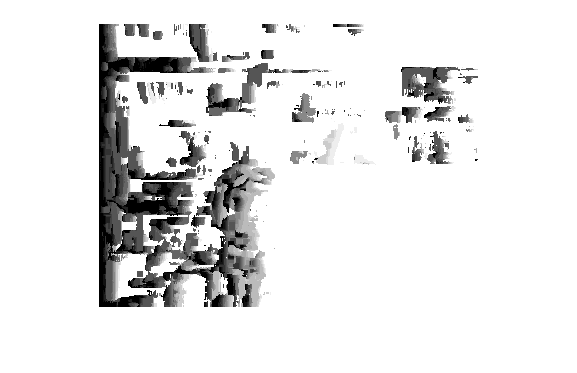
\includegraphics[width=\linewidth]{abs_dev15.png}
  \caption{Absolute difference}
  \label{fig1a}
 \end{subfigure}
 \begin{subfigure}{.49\textwidth}
  \centering
  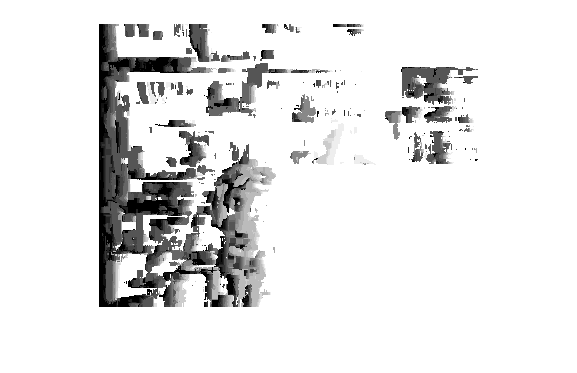
\includegraphics[width=\linewidth]{squared_dev15.png}
  \caption{Squared difference}
  \label{fig1b}
 \end{subfigure}
 \begin{subfigure}{.49\textwidth}
  \centering
  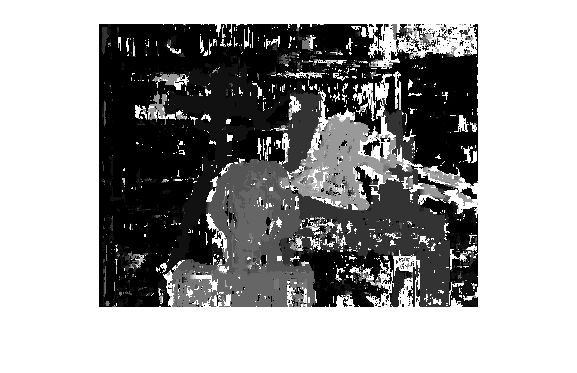
\includegraphics[width=1\linewidth]{corr_dev15.png}
  \caption{Correlation}
  \label{fig1c}
 \end{subfigure}
 \caption{Depth maps using the whole width as strip}
 \label{fig1}
\end{figure}

\subsection{Results}
For these results we used patch sizes of 15 by 15.

We started using strips of the full length of the width of the picture. Figure \ref{fig1} shows results for the absolute and squared difference and the correlation similarity measures. The figure shows quite poor results for the difference measures, while it shows reasonable results for the correlation similarity. The fact that it performs so bad for the difference measures probably has to do with the fact that often the algorithm finds a place in the image that has a large resemblance, but is very far away from the original place. This means that the image of course shows a lot of high pixel values. To avoid this problem we decided to use strips that do not cover the whole width of the image, but strips with as maximum width the maximum depth of the image with a small margin (15), which we determined in exercise 1. Moreover we shift the strip away from the pixel as much as the minimum depth of the image (5). Figure \ref{fig2} shows the results for these strips. As we can see these images show far better results for the difference measures, but the downfall to this method of course is that it needs a lot of human input. A human first has to determine the maximum and minimum depth of the image using manual techniques as we did in exercise 1, before the window of the strip can be determined. Moreover, we see that for the correlation similarity measures this method loses much of the noise that was present when using the whole strip, but it also blurs the edges to such an extent, that some contours are hard to distinguish.

\begin{figure}[ht!]
 \centering
 \begin{subfigure}{.8\textwidth}
  \centering
  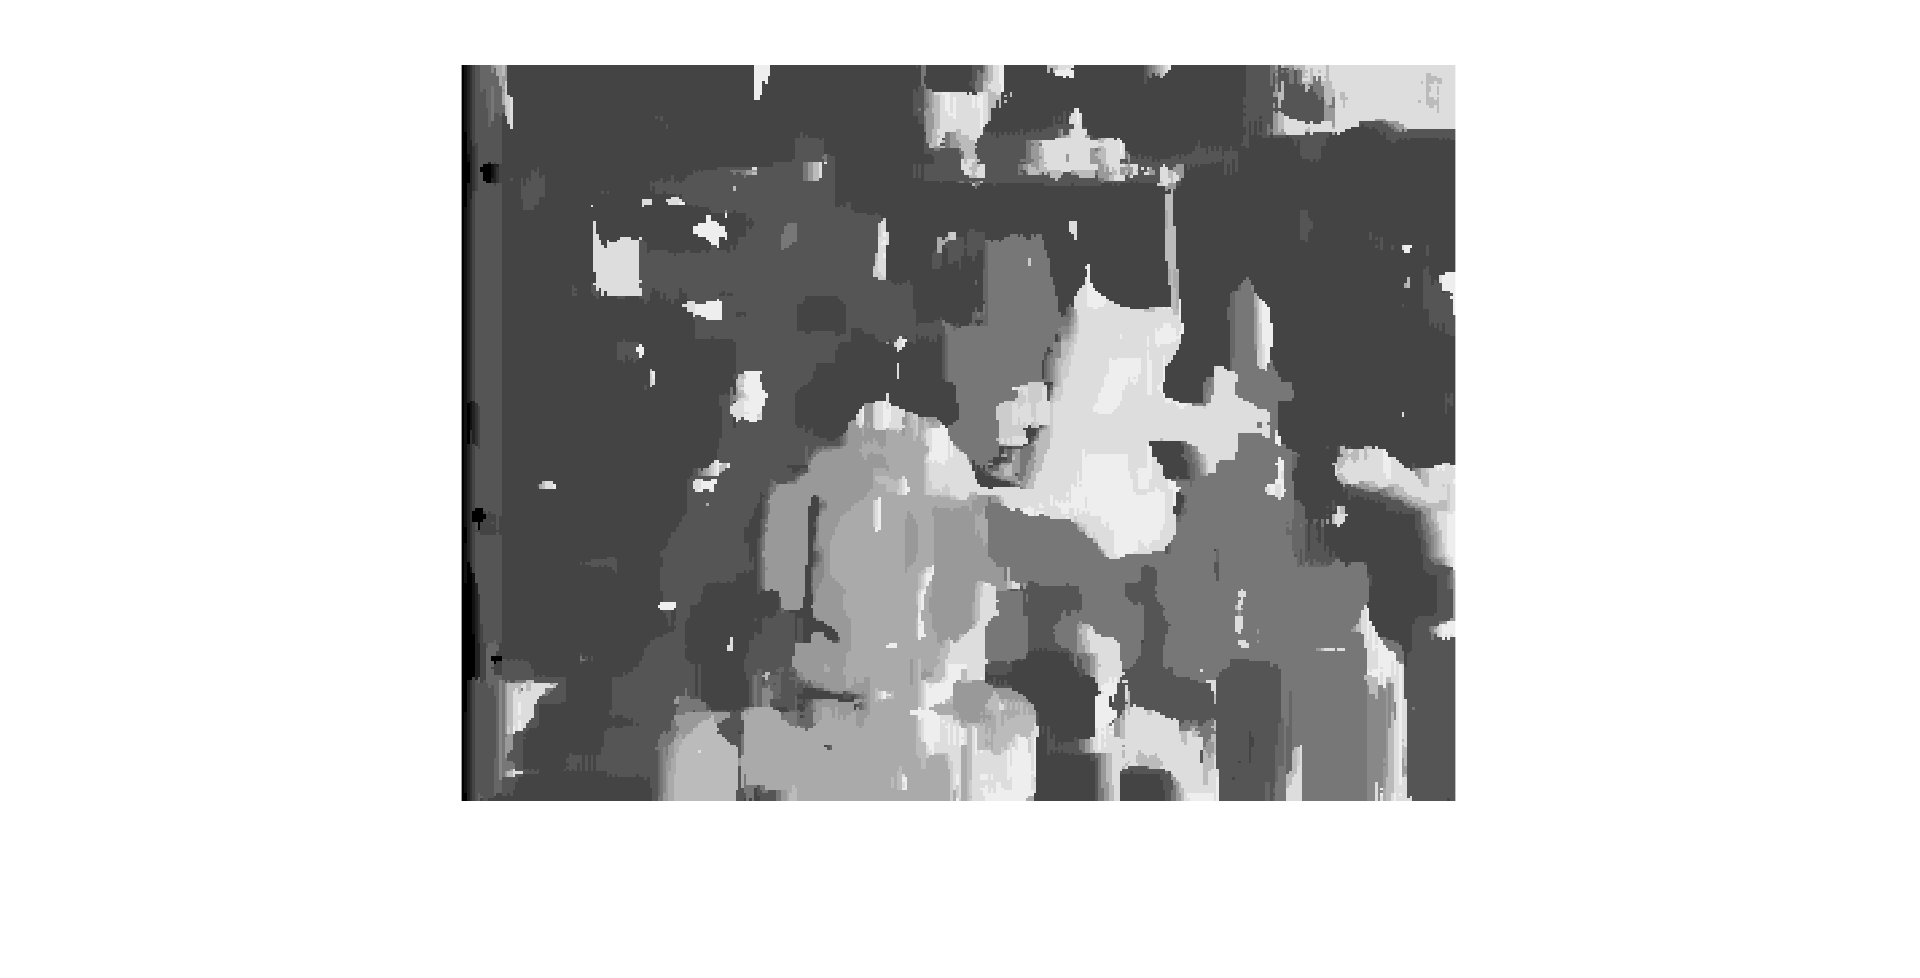
\includegraphics[width=1\linewidth]{abs_patch15.png}
  \caption{Absolute difference}
  \label{fig2a}
 \end{subfigure}
 \begin{subfigure}{.8\textwidth}
  \centering
  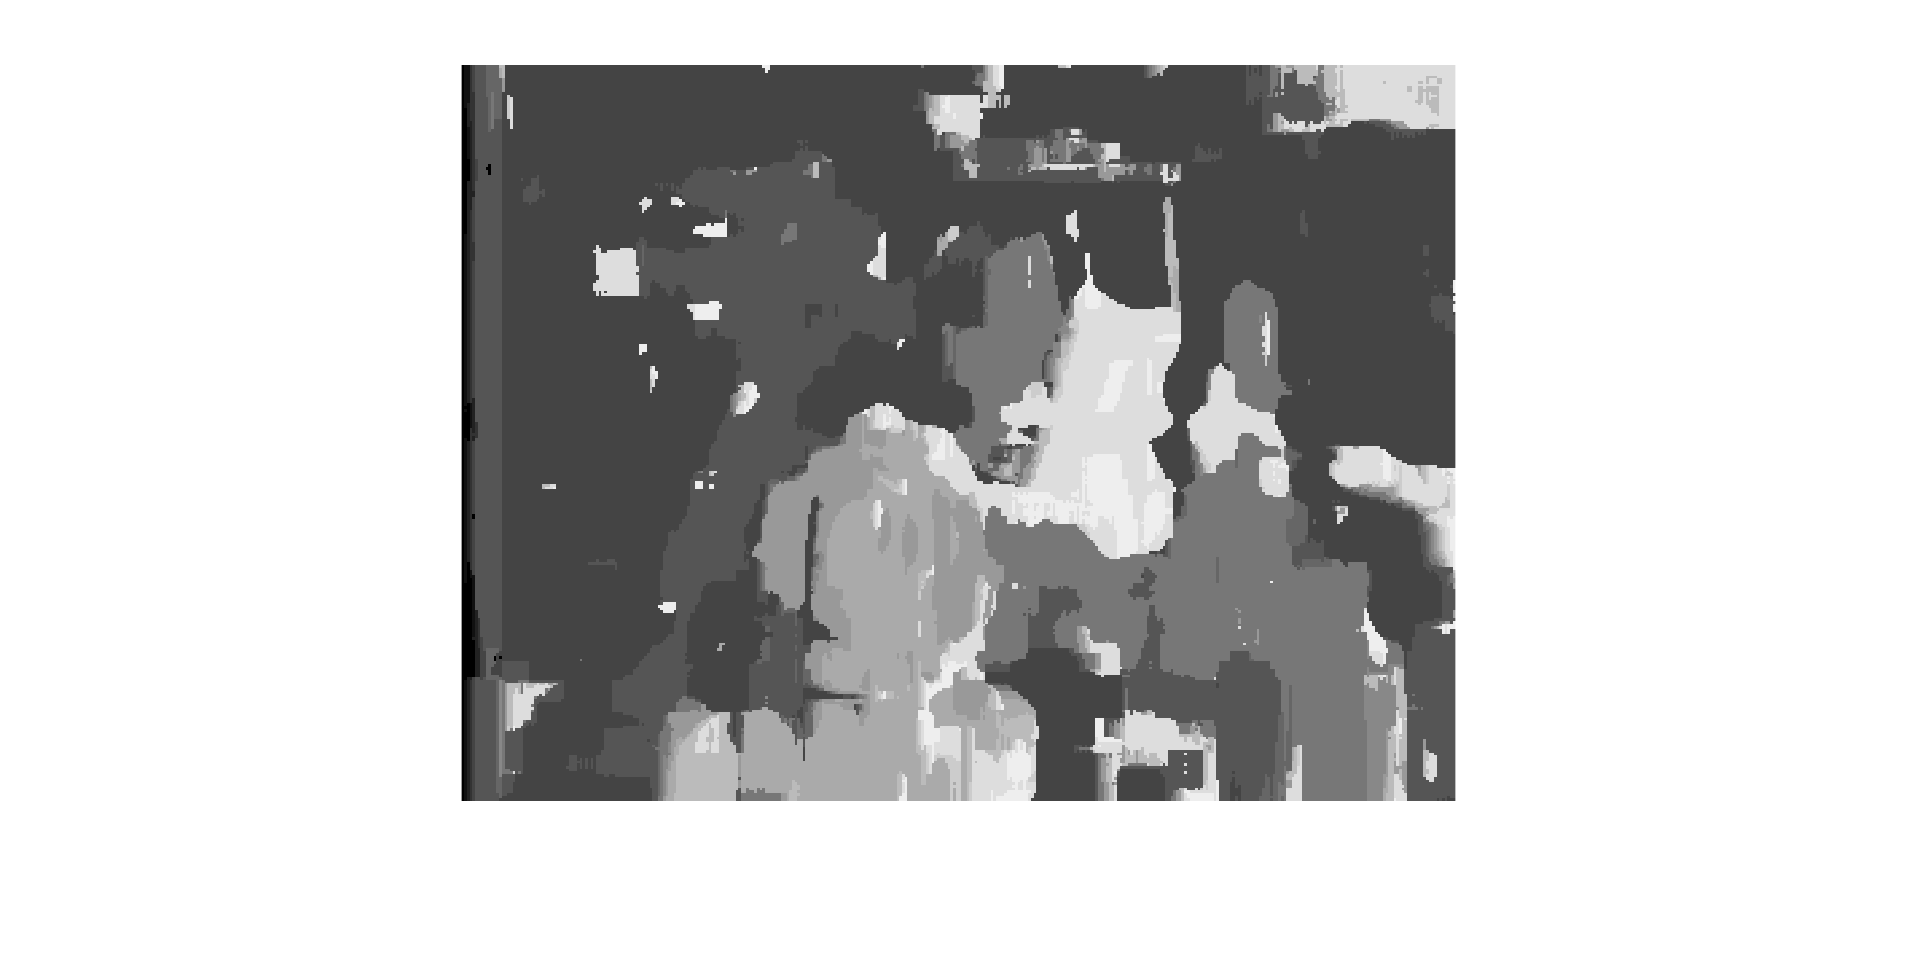
\includegraphics[width=1\linewidth]{squared_patch15.png}
  \caption{Squared difference}
  \label{fig2b}
 \end{subfigure}
 \begin{subfigure}{.8\textwidth}
  \centering
  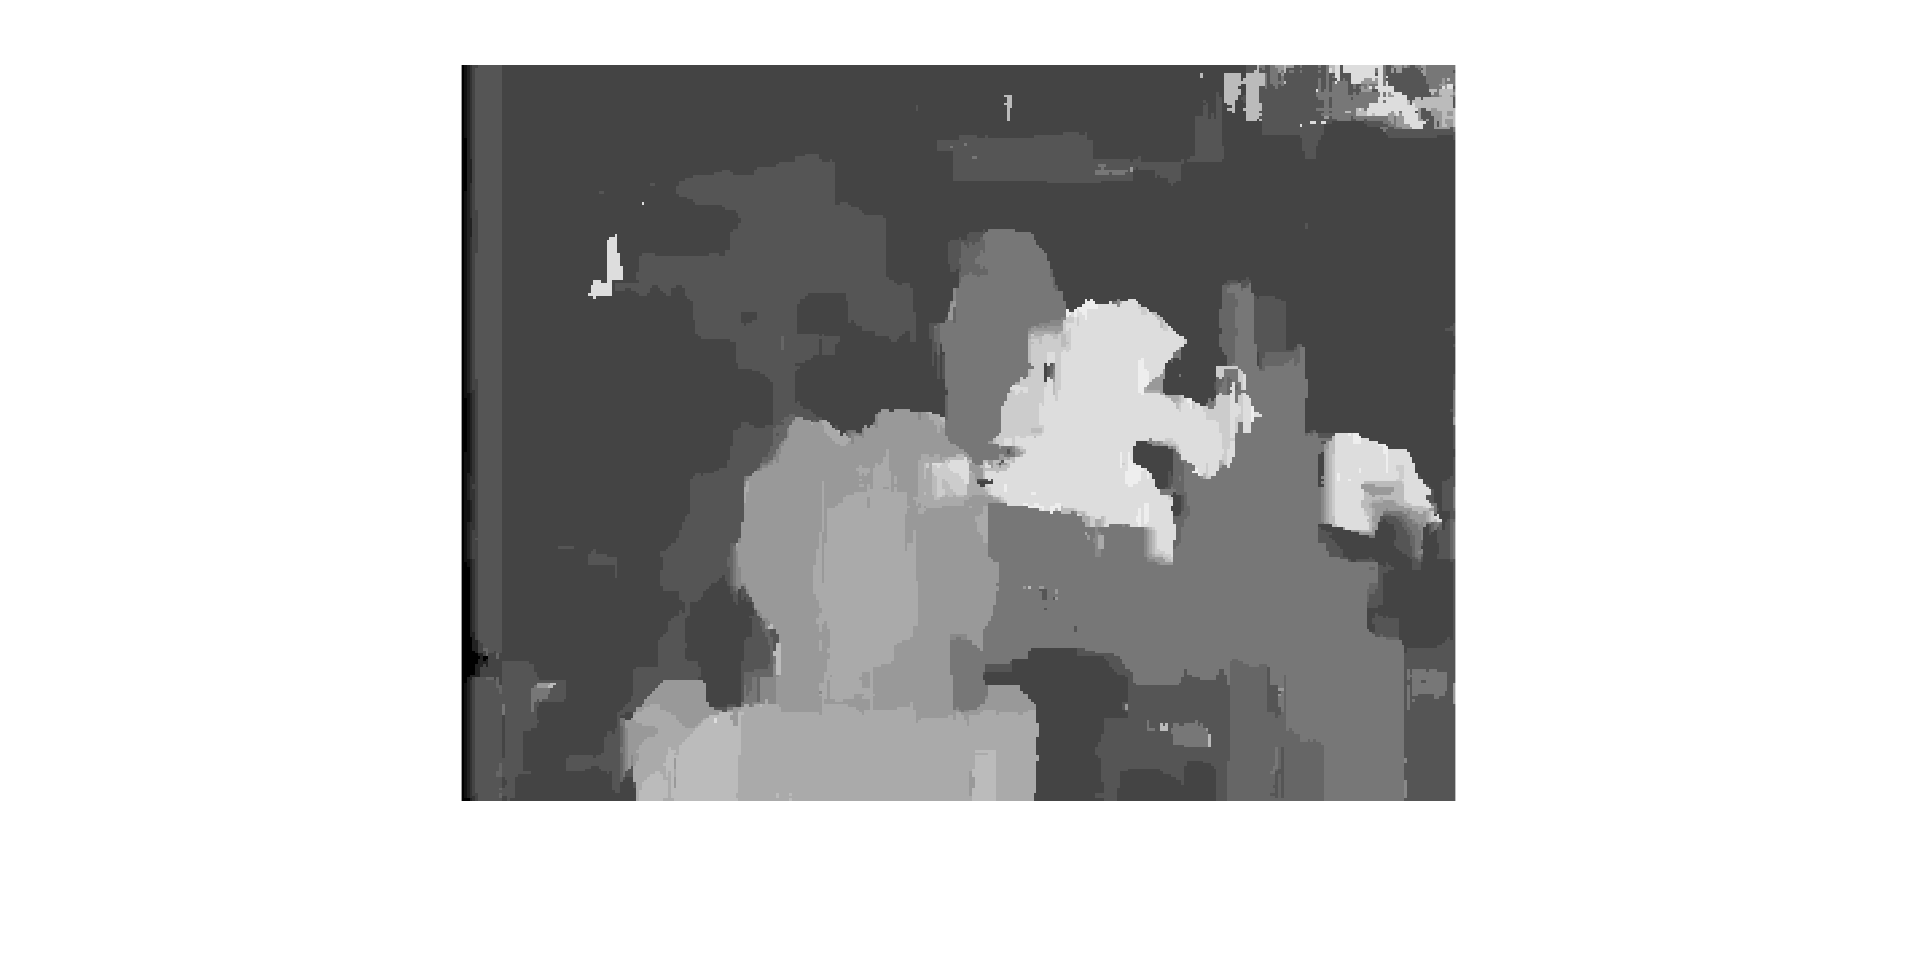
\includegraphics[width=\linewidth]{corr_patch15.png}
  \caption{Correlation}
  \label{fig2c}
 \end{subfigure}
 \caption{Depth maps using a strip of 5 to 15 difference in the x coordinate.}
 \label{fig2}
\end{figure}

Overall when we look at the differences in performance between the different similarity measures we can state that when we use the whole width (so when we are not `cheating'), the correlation measure by far outperforms the difference measures, since the latter do not distinguish the contours clearly at all. On the other hand when we `cheat' and use a fixed strip size, the performances differ less, but the correlation measure still performs better than the difference measures. 

\section{}


\section{}
To match the images using SIFT-features we first convert the image into grayscale images and then run the script given in appendix \ref{code:SIFT} (this uses a slightly adjusted \texttt{match.m}, which also returns the vector \texttt{match}). In this script we calculate the disparities between the matches that have a maximum difference of two y-pixels and store it together with the coordinates. Furthermore the y-differences and the number of equal y-values and the maximum y-value are stored.

Figure \ref{matches} shows the matches between the two images. As we can observe, the matches are all near-horizontal. However, if we look at the number of exactly equal y-values, this is only 20, so most of the matches do not seem to be at the exact same y-coordinate. However, we use as a criterium that the y coordinate can maximally differ 0.5 and of the 446 matches, 433 abide to this criterium. Since Sift somehow changes x-values into floating point numbers, this probably means that all of these 433 values are at the exact same y-coordinate in the actual image. The maximum y-difference however is 12.8, so this is definitely a false match.

The disparities that are calculated are in the same order as the test we did in exercise 1, with a maximum of 13.56 and a minimum of 2.95. We calculated the error based on the difference of disparity between every pixel corresponding to the a found SIFT feature and its corresponding pixel in the ground truth image (see appendix \ref{code:errorSIFT}. This yields the results given in table \ref{table2}. 

\begin{table}[!ht]
 \centering
 \caption{Total error of the 446 SIFT feature pixels compared to their corresponding pixels in the ground truth}
 \begin{tabular}{c|c}
 Method & Error \\
 \hline
 SIFT & 152 \\
 Absolute difference & 148 \\
 Correlation & 144
 \end{tabular}
 \label{table2}
\end{table}
The table shows that the SIFT method has the largest total error and the windowing methods have the smaller errors, with the correlation method performing best. The differences do not seem significant however, so it would be necessary to run this comparison for more images than just this one. 

\begin{figure}[ht!]
 \centering
 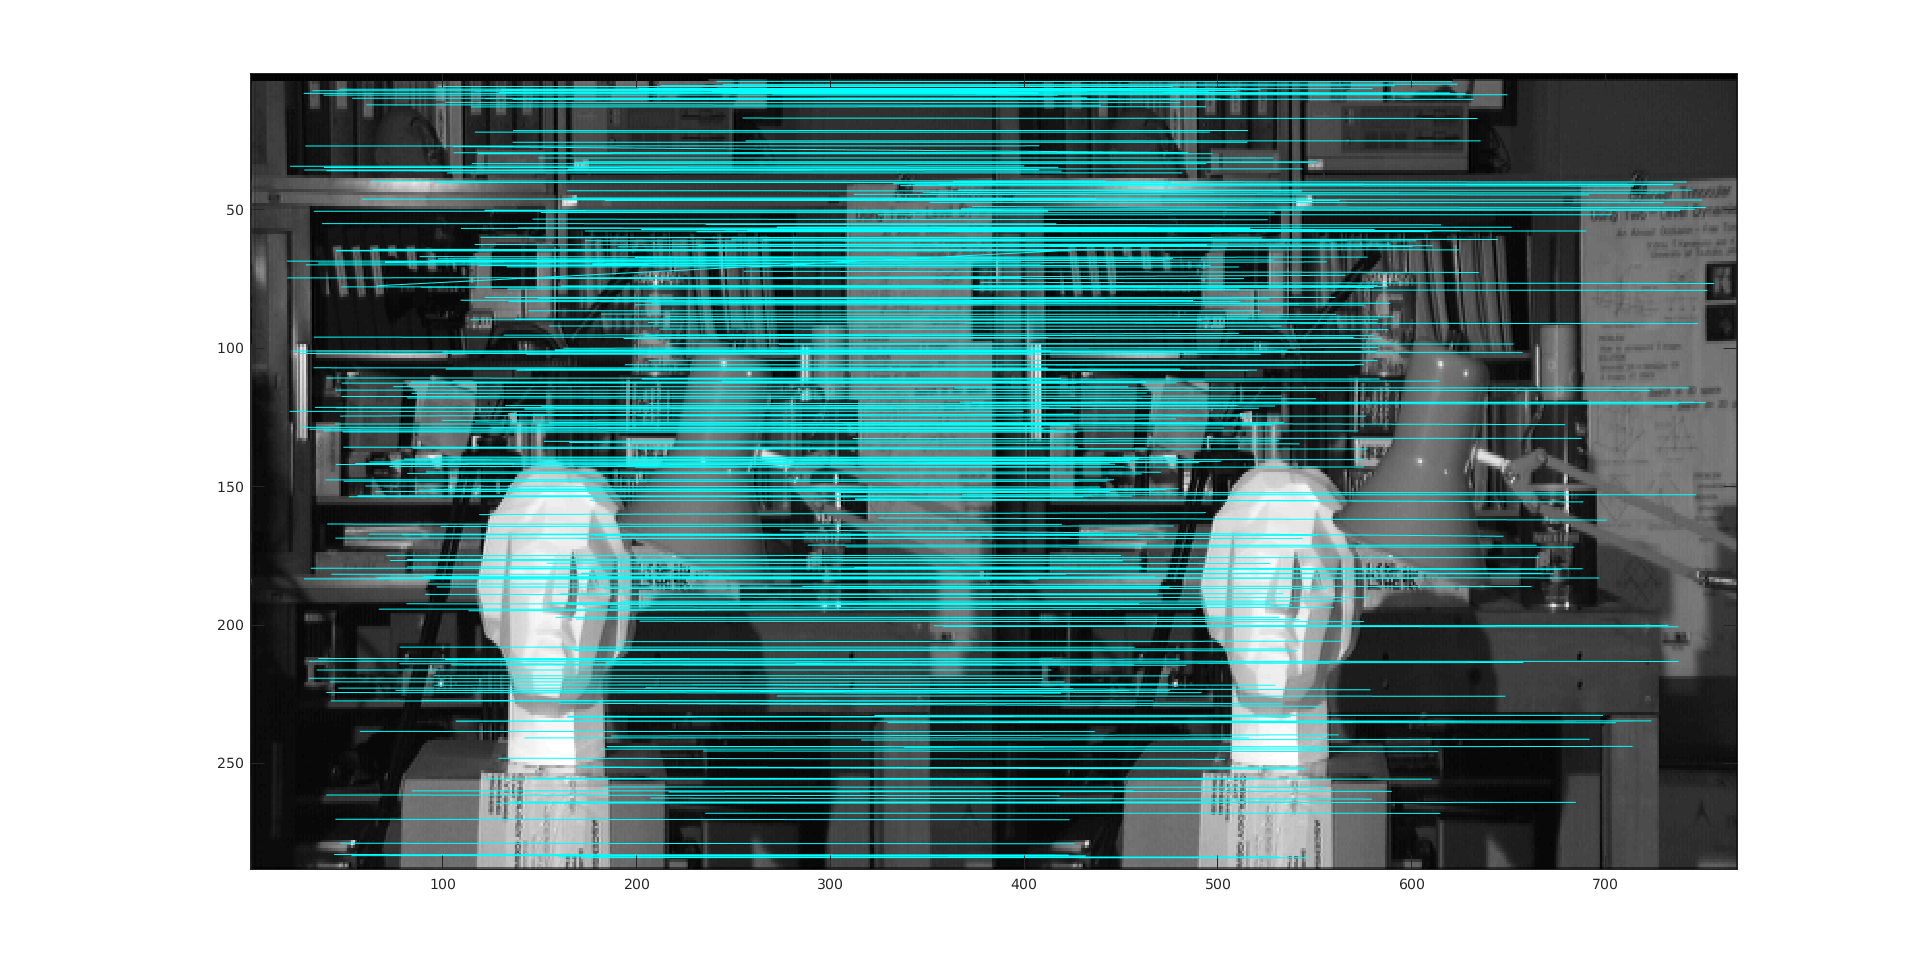
\includegraphics[width = \linewidth]{matches.png}
 \caption{The found matches between the two images by using SIFT features}
 \label{matches}
\end{figure}

\begin{appendices}
\section{Code}
\lstinputlisting[caption={depthmap.m},label={code:depthmap}]{../stereoprakt/depthmap.m}
\lstinputlisting[caption={absdiff.m},label={code:absdiff}]{../stereoprakt/absdiff.m}
\lstinputlisting[caption={squareddiff.m},label={code:squareddiff}]{../stereoprakt/squareddiff.m}
\lstinputlisting[caption={xcorrdiff.m},label={code:xcorrdiff}]{../stereoprakt/absdiff.m}
\lstinputlisting[caption={Script to determine the disparities using SIFT-features},label={code:SIFT}]{../SIFT/stereoSift.m}
\lstinputlisting[caption={errorSIFT.m},label={code:errorSIFT}]{../stereoprakt/errorSIFT.m}
\end{appendices}

\end{document}